\documentclass[12pt]{standalone}


\usepackage{amssymb} 
\usepackage{amsmath} 

\usepackage[no-math]{fontspec}
\usepackage{unicode-math}
\setmainfont{TeX Gyre Heros}
\setmathfont{Stix Two Math}

\usepackage{tikz}
\usetikzlibrary{arrows.meta, backgrounds}

\usepackage{xcolor}
\definecolor{itwm_blue_04}{HTML}{005A94}
\definecolor{bgcolor}{HTML}{f3f4f4}

\usepackage{nicefrac}


\begin{document}
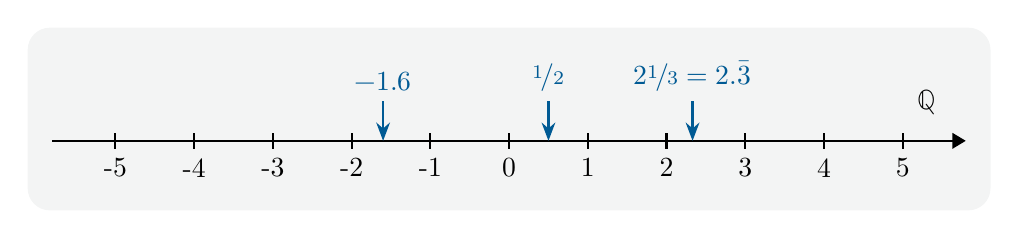
\begin{tikzpicture}[
    show background rectangle,
    background rectangle/.style={fill=bgcolor, rounded corners=8pt},
    inner frame sep=0.3cm
]
%
\draw [-{Triangle}, thick] (-5.8,0) -- (5.8,0);
\foreach \x in {-5,...,5} {
    \draw [thick] (\x,-.1) -- (\x,0.1);
    \node[below] at (\x,-0.1) {\x};
}
\draw [itwm_blue_04, thick, -{Stealth}] (-1.6,0.5) node [above] {$-1.6$} -- (-1.6,0);
\draw [itwm_blue_04, thick, -{Stealth}] (0.5,0.5) node [above] {$\nicefrac{1}{2}$} -- (0.5,0);
\draw [itwm_blue_04, thick, -{Stealth}] (2.33,0.5) node [above] {$2\nicefrac{1}{3} = 2.\bar{3}$} -- (2.33,0);
\node[above] at (5.3,0.2) {$\mathbb{Q}$};
\end{tikzpicture}
\end{document}